\chapter{Design of Demo Devices}
This chapter is focused on the tag reader and power control device of the \textbf{Parentsystem}. 
The design and functionality of the prototype will be presented in parallel to the designed end product.

\section{Product Design}

There is two devises need to activete a usage of device from the user to the server as shown in figure below.

\begin{figure}[h]
	\centering
		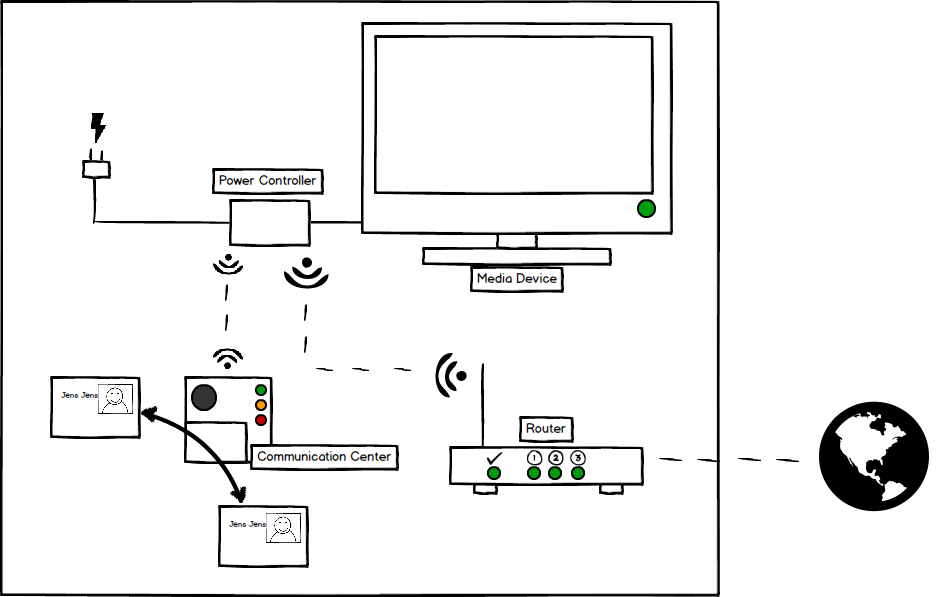
\includegraphics[width=1.00\textwidth]{images/Power&Tagdevice.png}
	\caption{Rich picture for Powercontrol and Tag reader}
	\label{fig:Power&Tagdevice}
\end{figure}

One is a small detection device to read user tags when swiped over it, this devise is often placed in the most asseble place. 
The other devise is a powercontrol devise whitch i located on the powerline to the media device and tunes on and off the electrisity when needed.
The powercontrol devise(PCD) is the brain of the two devises and is therefore to moniter the users time usage and communication center with the server and detection devise. 
The detection devise(DD) also work as infomation communicater to the user on the state of the connection to the server, acceptens/decline of login and more.     

\subsection{Senario Design}

The systemt is designed on mulitble senarios and the creteria of communication to server and user. The flow chart below is a overview of actions and communication the two devices have to give the right permission to user, communicat with the user and server about status, handel disconnection to server and control of user- and timeusage restrictions.

\fixme{indsæt Flowcart af systemet}

To test develop the flowcart of the system is multible usercases constucted.


\textbf{Setting up and turning on the system.} \n
The PCD retive information on wifi connection form USB port if an USB is connected at start point of PCD. 
If the USB information is wrong or not retived then a restart botton is included to redo the procedure.  \n
The PCD will then connect to the wifi network and to the web server of MOM. If the connection isn't found a massage is send to the DD. \n DD indicate that there is no connection by showing a constant red light. The communication protocal can be found in the appendix  \fixme{indsæt referance til appendix table af lys indikater}.\n When the connection is established then the DD is ready to read user tags.

\textbf{Detection of connection issues and status changes.} \n
The connection to the sever is tested by a rutine call every five minutes form the PCD to the server. In this call will the PCD recieve information on when next rule or user time cut will come. This both insure that there is connection each five minutes and if any changes in rules or in the time the user may spend on the media device. In the period between the call will the PCD ask for a tag from the DD. If the PCD is disconnected form the server that is informed to the DD and to the user.  
	
\textbf{Logon/logoff media divice.} \n
When a tag is read by the DD will the PCD recieve the tag id which formed to a login massage if no one is all ready logged in the system. The PCD will then read if the user is declined or accepted to use the device. If the user is accepted then the PCD will switch the power on to the media device, save the tag id in local memory and recieve time left before a rule or to time usage limit accour. The DD indicate to the user that he/she is approved to use the media device.\n When the PCD recieve the tag id that is stored in the local memory then it means the user is logging off. The PCD will switch off the power to the media device and send a logoff massage til the server. Should another user want to take over the usage of a media device the PCD will try to login with the new tag if declined then the DD will then signal this and keep the old user on. If accepted then the server will overwirte the the previus user and PCD will recieve the information for the new user with out turning the power off and then on again.


\textbf{Disconnection under use.} \n
A disconection is either found under the regular status call efter each five minutes or at a logon/logoff call. A disconection will lock the device so only the current user can use the media device until the PCD is reconected with the server. The server see the disconection when there haven't been a status call from the device in five minutes. The disconnection is translated to a logoff at the server side stoppe the usage of the users time to use media devises. The use will not be logged off at the media device but will be able to use his/her time until a rule or his/her time used up according to the last status the PCD have got and is keeping track of. If the user want to logoff in a period where there is a disconnection a time stamp is set to sent to the server when the connection is reastablage. The media can also first be used when the connection is reastablage.   
This procedure have the advange that the user will not have to cut off the media in use if the connection is waopely and the user will be able to login on other media device even with previus media divice not yet have connection. 
The disavenge is that the user has the possiblety to overuse the time resigtion by still use the disconnected divice until there is no more time and in the mean time has turned on at new device. 
The disadvange will but also have the effect to punish the user with a big negitive time to use other devices when the disconnected device is reconnected and this should discourage this senario.       
    
		
\section{Prototype Implemtation}
The prototype is designed to prove the concept of a tag reader and the communication protecal between powercontrol and server. Therefor shall the Ardurino hardware be seen as replaceble for to manufature this system it is need be unic devices that is able to connect on the power core to the the media device and slim designed card reader with speaker and indications lights. To prove the conecpt the device is able to read and accept/decline tags, indicate this using ligts to the user and turn on the power if accepteted.   




    